% homework/hw08/hw08.tex
% Year 7 - Homework Packet 8: Where It Lands on the Line.
%
% Covers Science 2.8 (acids, bases, indicators, the pH scale, neutralisation),
% a short Science 2.7 block (compounds and mixtures), Mathematics 2.6
% (inequalities), 2.5 (equations and formulae) and 3.1-3.2 (place value and
% rounding).
%
% THE SPINE IS THAT EVERY SCALE ON THE PACKET IS THE SAME OBJECT. The pH scale
% is a number line you put a liquid on. An inequality is a number line with a
% circle on it. A measuring cylinder is a number line stood on its end. A graph
% axis is two of them. Rounding is deciding which mark on the line you are
% allowed to land on. Section F says this out loud; Sections A and C act it out
% on one set of eleven liquids, first in science and then in maths.
%
% Three ties are exact rather than decorative:
%   * C2 reads Section A's pH table with < and >. Four of its six inequalities
%     turn on the open-circle rule, because every pH on the list is a decimal
%     and four of them are named exactly (p > 9.6 excludes baking soda at 9.6;
%     p > 12.6 excludes bleach at 12.6 and so has NO answer at all). Pure water
%     at 7.0 is in neither p < 7 nor p > 7.
%   * F2's cylinders A and B are the SAME PICTURE with different numbers, and
%     the two readings are 65 and 6.5 -- a factor of ten, which is Section E.
%   * F3(f) asks for the formula of the graph's line, and that formula,
%     m = 60 + v, is D3(e). The graph is the formula drawn.
%
% Nothing here is lifted from the workbook. Where a trap from a deck is reused
% it has new numbers and a new context. The pH values are the deck's own
% (Science 2.8, slide 14) with a decimal added, so the scale the class coloured
% in their notebooks and the scale on this packet still agree while A1 stops
% being a lookup. A1 gives the number and asks for the place; F2 and F3 give
% the place and ask for the number. They are inverses, and Section F's opening
% line says so.
%
% House style is shared: see homework/hw-style.tex. Method: the new-homework
% skill. Source is pure ASCII on purpose.
%
% Build:  pwsh .claude/skills/new-homework/scripts/build-hw.ps1 hw08

\documentclass[12pt,a4paper]{article}

% -- Answer key switch -------------------------------------------------------
\newif\ifkey
\ifdefined\TEACHER\keytrue\else
  \keyfalse        % \keyfalse = student copy   |   \keytrue = teacher copy
\fi

% -- House style -------------------------------------------------------------
% homework/hw-style.tex
% Shared house style for every Year 7 homework packet. \input this from the
% packet file, right after \documentclass and the answer-key switch.
%
% Do not fork this file per packet. If a packet needs a different look, the
% question is whether every packet should have it.
%
% The choices here are deliberate and were arrived at by printing and looking:
%   * No solid dark banners. Every header is a light tint with a coloured spine
%     on the left, so colour reads clearly without flooding a school printer.
%   * No marks and no mark totals. These are practice, not exam papers.
%   * Lato at 12pt with open leading, plus mathastext so inline maths is Lato
%     too. Without mathastext every "-6 + 4" is Computer Modern serif and the
%     sheet looks half-typeset.
%   * Writing lines are spaced for Year 7 handwriting, not adult margin notes.
%
% Provides: \wlines \blank \tickbox \sep \qmk-free marks (none) \hwsection
% \qhead \expr, the workspace box, and the remember / wordhelp / activity /
% yourturn coloured boxes. Palette matches the lesson decks exactly.

% -- Packages ----------------------------------------------------------------
\usepackage[T1]{fontenc}
\usepackage[utf8]{inputenc}
\usepackage[default]{lato}
\usepackage[a4paper,top=1.7cm,bottom=1.7cm,left=2.0cm,right=2.0cm,headheight=15pt]{geometry}
\usepackage{amsmath,amssymb}
\usepackage{xcolor}
\usepackage[most]{tcolorbox}
\usepackage{enumitem}
\usepackage{tikz}
\usetikzlibrary{arrows.meta}
\usepackage{array}
\usepackage{tabularx}
\usepackage{fancyhdr}
\usepackage{multicol}
\usepackage{needspace}
\usepackage{graphicx}

% Make maths use Lato too. Without this, every "-6 + 4" on the page is set in
% Computer Modern serif and the sheet looks half-typeset. Must come last.
\usepackage[italic]{mathastext}

\linespread{1.06}\selectfont

% -- The Learner's Book palette (same hex values as the lesson decks) ---------
\definecolor{cbteal}{HTML}{0087A8}
\definecolor{cbpurple}{HTML}{5C2483}
\definecolor{cborange}{HTML}{C25E12}
\definecolor{cbgreen}{HTML}{4A8B23}
\definecolor{cbred}{HTML}{C8102E}
\definecolor{cbblue}{HTML}{1A5FA8}
\definecolor{rulegray}{HTML}{9AA5AD}

% -- Answer lines and blanks -------------------------------------------------
% \wlines{n} draws n ruled writing lines, spaced wide enough for Year 7
% handwriting rather than for an adult with a fine pen.
\makeatletter
\newcommand{\wlines}[1]{%
  \par\vspace{0.75em}%
  \@tempcnta=0\relax
  \@whilenum\@tempcnta<#1\do{%
    \hbox to \linewidth{\color{rulegray}\leaders\hrule height 0.5pt\hfill}%
    \vspace{1.5em}%
    \advance\@tempcnta by 1\relax}%
  \par\vspace{-0.8em}%
}
\makeatother

% \blank[width] is an inline gap to write a short answer in.
\newcommand{\blank}[1][2.6cm]{\underline{\hspace{#1}}}

% A boxed space for showing working.
\newtcolorbox{workspace}[1][3.4cm]{%
  colback=white, colframe=rulegray, boxrule=0.5pt, arc=5pt,
  height=#1, left=6pt, right=6pt, top=4pt, bottom=4pt,
  before skip=9pt, after skip=11pt}

% An empty tick box.
\newcommand{\tickbox}{\fbox{\rule{0pt}{1.15em}\rule{1.15em}{0pt}}}

% A middot separator.
\newcommand{\sep}{\,\textperiodcentered\,}

% -- Section and question headings -------------------------------------------
% Light tint plus a fat coloured spine on the left. No solid dark banner: the
% colour reads clearly but barely costs the printer anything.
% needspace stops a heading stranding alone at the foot of a page. Kept modest:
% too large and it pushes headings over, leaving a worse hole than it prevents.
\newcommand{\hwsection}[2][cbteal]{%
  \needspace{8\baselineskip}%
  \par\vspace{13pt}%
  \noindent
  \begin{tcolorbox}[enhanced, nobeforeafter, width=\textwidth,
      colback=#1!7, colframe=#1!7, arc=5pt,
      borderline west={5pt}{0pt}{#1},
      left=14pt, right=10pt, top=7pt, bottom=7pt]
    {\large\bfseries\color{#1}#2}
  \end{tcolorbox}%
  \par\vspace{9pt}}

% \qhead[colour]{A2}{Moving along the line} -- a question heading.
\newcommand{\qhead}[3][cbteal]{%
  \needspace{6\baselineskip}%
  \par\vspace{11pt}%
  \noindent{\large\bfseries\color{#1}#2}\quad{\large\bfseries #3}\par\vspace{4pt}}

% -- Coloured boxes ----------------------------------------------------------
% Shared look: rounded, light fill, coloured rule, coloured title text on a
% pale title strip rather than a dark one.
\tcbset{hwbox/.style={
  enhanced, breakable, arc=6pt, boxrule=1pt,
  left=11pt, right=11pt, top=8pt, bottom=8pt,
  fonttitle=\bfseries, attach boxed title to top left={xshift=12pt, yshift=-8pt},
  boxed title style={arc=4pt, boxrule=1pt, left=7pt, right=7pt, top=2pt, bottom=2pt},
  top=13pt}}

% Orange: things to remember. Matches the deck's "Write This Down".
\newtcolorbox{remember}[1][Remember from the lesson]{hwbox,
  colback=cborange!6, colframe=cborange, coltitle=cborange,
  colbacktitle=white, title={#1}}

% Blue: English help. The barrier in this class is the wording, not the maths.
\newtcolorbox{wordhelp}[1][Word help]{hwbox,
  colback=cbblue!6, colframe=cbblue, coltitle=cbblue,
  colbacktitle=white, title={#1}}

% Purple: an activity or instruction.
\newtcolorbox{activity}[1][How to do this homework]{hwbox,
  colback=cbpurple!6, colframe=cbpurple, coltitle=cbpurple,
  colbacktitle=white, title={#1}}

% Green: your turn / a friendly nudge.
\newtcolorbox{yourturn}[1][Your turn]{hwbox,
  colback=cbgreen!7, colframe=cbgreen, coltitle=cbgreen!75!black,
  colbacktitle=white, title={#1}}

% -- Shorthands --------------------------------------------------------------
\newcommand{\dC}{\,^{\circ}\mathrm{C}}          % use inside maths: $-8\dC$
\newcommand{\key}[1]{{\color{cborange}\textbf{#1}}}
\newcommand{\eng}[1]{{\color{cbblue}\textbf{#1}}}

\setlist[enumerate]{itemsep=8pt, topsep=5pt, leftmargin=*}
\setlist[itemize]{itemsep=4pt, topsep=4pt, leftmargin=*}
\renewcommand{\arraystretch}{1.45}

% -- An expression the student is asked to work from -------------------------
\newcommand{\expr}[1]{%
  \tcbox[on line, colback=cbgreen!10, colframe=cbgreen!55, boxrule=1pt, arc=4pt,
         left=9pt, right=9pt, top=4pt, bottom=4pt]{\large\bfseries $#1$}}

% -- Running head and foot ---------------------------------------------------
% The packet overrides \fancyhead[L] with its own title.
\pagestyle{fancy}
\fancyhf{}
\fancyhead[L]{\small\color{black!55}Year 7\sep Homework}
\fancyhead[R]{\small\color{black!55}Name: \blank[3.4cm]}
\fancyfoot[C]{\small\color{black!55}Page \thepage}
\renewcommand{\headrulewidth}{0pt}
\renewcommand{\headrule}{\vspace{2pt}\hbox to\headwidth{\color{cbteal!45}\leaders\hrule height 1.2pt\hfill}}



% -- Per-packet running head -------------------------------------------------
\fancyhead[L]{\small\color{black!55}Year 7\sep Homework 8}

% -- A group of writing lines that will not be split -------------------------
% See hw06.tex: \wlines is a run of separate hboxes and TeX will break in the
% middle of one, stranding a single rule at the top of the next page.
\newcommand{\qlines}[1]{\par\needspace{\numexpr#1+1\relax\baselineskip}\wlines{#1}}

% -- A chemical formula ------------------------------------------------------
% Upright, so it does not come out in mathastext's italic and read as algebra.
\newcommand{\ch}[1]{\ensuremath{\mathrm{#1}}}

% -- A box to write one number in --------------------------------------------
\newcommand{\nbox}{\ \fbox{\rule{0pt}{1.05em}\rule{1.0em}{0pt}}\ }

% -- An answer blank that will not cause an overfull line ---------------------
% "\hfill \blank[3.4cm]" at the end of a wrapping \item overflows the margin
% when the text happens to fill its last line. \ansline puts the blank on a
% line of its own, right-aligned, which cannot overflow.
\newcommand{\ansline}[1][4.4cm]{\par\vspace{2pt}\hspace*{\fill}\blank[#1]\par}

% -- A cubic centimetre ------------------------------------------------------
\newcommand{\ccm}{\ensuremath{\mathrm{cm^3}}}

% -- A ragged-right X column -------------------------------------------------
% Justified prose in a 4 cm table cell stretches the interword spaces until the
% row reads as three separate words. Every X column holding words uses this.
\newcolumntype{L}{>{\raggedright\arraybackslash}X}

% -- "h = ______", right-aligned, on a line of its own -----------------------
% Same reason as \ansline: "\hfill $h = \blank$" at the end of a wrapping \item
% strands the "h =" at the right margin and drops the blank to the next line,
% which is what D3(d) and D3(e) did.
\newcommand{\ansfor}[2][2.8cm]{\par\vspace{1pt}\hspace*{\fill}$#2 = \blank[#1]$\par}

% ---------------------------------------------------------------------------
% UNIVERSAL INDICATOR, pH 1 AT THE LEFT TO pH 14 AT THE RIGHT.
% These are the exact hex values the lesson deck uses (Science 2.8,
% diagrams.js), so the scale the class coloured into their notebooks on slide
% 13 and the scale printed here are the same scale. Do not "improve" them.
% The names are pHa..pHn: a bare letter such as \l or \c would collide with a
% LaTeX accent command the moment it became a \foreach variable.
% ---------------------------------------------------------------------------
\definecolor{pHa}{HTML}{D7191C}
\definecolor{pHb}{HTML}{E8462C}
\definecolor{pHc}{HTML}{F06E28}
\definecolor{pHd}{HTML}{F79B2C}
\definecolor{pHe}{HTML}{FAC432}
\definecolor{pHf}{HTML}{ECDF2A}
\definecolor{pHg}{HTML}{4CAF50}
\definecolor{pHh}{HTML}{24A58C}
\definecolor{pHi}{HTML}{1F8AC0}
\definecolor{pHj}{HTML}{1F6BB5}
\definecolor{pHk}{HTML}{2F4FA3}
\definecolor{pHl}{HTML}{4A2F96}
\definecolor{pHm}{HTML}{63258C}
\definecolor{pHn}{HTML}{7A1F7A}

% -- A number line, blank, from #1 to #2 -------------------------------------
\newcommand{\numline}[2]{%
  \begin{tikzpicture}[x=0.84cm, y=0.84cm, line width=0.9pt]
    \draw[cbteal,{Latex[length=2.8mm]}-{Latex[length=2.8mm]}]
      ({#1-0.7},0) -- ({#2+0.7},0);
    \foreach \n in {#1,...,#2}{
      \draw[cbteal] (\n,-0.16) -- (\n,0.16);
      \node[below=2pt, font=\small] at (\n,-0.16) {$\n$};}
  \end{tikzpicture}}

% -- A number line with an inequality already shown on it --------------------
% #1 from, #2 to, #3 the open circle, #4 where the arrow ends.
\newcommand{\numlinemark}[4]{%
  \begin{tikzpicture}[x=0.84cm, y=0.84cm, line width=0.9pt]
    \draw[cbteal,{Latex[length=2.8mm]}-{Latex[length=2.8mm]}]
      ({#1-0.7},0) -- ({#2+0.7},0);
    \foreach \n in {#1,...,#2}{
      \draw[cbteal] (\n,-0.16) -- (\n,0.16);
      \node[below=2pt, font=\small] at (\n,-0.16) {$\n$};}
    \draw[cborange, line width=1.9pt, -{Latex[length=3.2mm]}] (#3,0.46) -- (#4,0.46);
    \draw[cborange, line width=1.4pt, fill=white] (#3,0.46) circle (0.17);
  \end{tikzpicture}}

% -- One measuring cylinder --------------------------------------------------
% #1 x shift, #2 its letter, #3 the numbered lines as "division/label, ...",
% #4 the water height in small divisions (0 draws an empty cylinder).
% Twenty small divisions, always. What changes between cylinders is only which
% lines carry a number and what those numbers say -- which is the whole of F2.
\newcommand{\cyl}[4]{%
  \begin{scope}[shift={(#1,0)}]
    \ifnum#4>0
      \fill[cbteal!22] (0.07,0.05) rectangle (1.53,#4);
      \draw[cbteal!80!black, line width=1.0pt]
        (0.07,#4) .. controls (0.55,{#4-0.6}) and (1.05,{#4-0.6}) .. (1.53,#4);
    \fi
    \draw[black!70] (0,21) -- (0,0) -- (1.6,0) -- (1.6,21);
    \draw[black!70] (-0.3,-1.1) -- (1.9,-1.1) -- (1.6,0) -- (0,0) -- cycle;
    \foreach \v in {1,...,20}{\draw[black!70, line width=0.7pt] (0,\v) -- (0.34,\v);}
    % The numbers go OUTSIDE, on the left. Printed on the glass as a real
    % cylinder has them, the 60 on A and the 6 on B land exactly on the
    % meniscus and the reading is unreadable at the one place it matters.
    \foreach \v/\lab in {#3}{
      \draw[black!70, line width=1.0pt] (0,\v) -- (0.66,\v);
      \node[anchor=east, font=\scriptsize] at (-0.14,\v) {\lab};}
    \node[font=\bfseries] at (0.8,22.6) {#2};
  \end{scope}}

\begin{document}

% ===========================================================================
% COVER BLOCK
% ===========================================================================
\thispagestyle{fancy}

\begin{tcolorbox}[enhanced, colback=cbpurple!7, colframe=cbpurple!7, arc=7pt,
                  borderline west={6pt}{0pt}{cbpurple},
                  left=18pt, right=14pt, top=10pt, bottom=10pt]
  {\color{cbpurple}\bfseries YEAR 7\sep UNITS 2 AND 3\sep HOMEWORK 8}\\[5pt]
  {\color{cbpurple}\Huge\bfseries Where It Lands on the Line}\\[7pt]
  {\color{black!70}Science 2.8 and 2.7 --- the pH scale; compounds and mixtures}\\
  {\color{black!70}Mathematics 2.6, 2.5 and 3.1--3.2 --- inequalities, equations, rounding}\\
  {\color{black!70}Section F --- the pH scale, the cylinder and the graph are one thing}
\end{tcolorbox}

\vspace{4pt}
\noindent
\begin{tabularx}{\textwidth}{@{}X X@{}}
  \textbf{Name:} \blank[5.6cm] & \textbf{Class:} \blank[5.6cm] \\
  \textbf{Date given:} \blank[4.6cm] &
  \textbf{Date due:} {\color{cbred}\bfseries Monday 28 September 2026} \\
\end{tabularx}

\vspace{2pt}
\begin{activity}
  Six sections. Science first this time: the maths in Section C reads the science
  table in Section A.
  \begin{itemize}
    \item In science, write \key{full English sentences}. ``Acid'' is not a
          sentence; ``Lemon juice is an acid because its pH is below 7'' is.
    \item In maths, \key{write the equation before you write the answer.}
          \eng{No calculator}, except where Section E says so.
  \end{itemize}
\end{activity}

% ===========================================================================
% SECTION A -- SCIENCE 2.8
% ===========================================================================
\hwsection{Section A \textperiodcentered\ Science 2.8 --- Acids, Bases and the pH Scale}

% -- A1 ---------------------------------------------------------------------
% The way in, and it is meant to be easy: put a letter in a box. A student who
% can start nothing else can start this. The instruction line comes BEFORE the
% word-help box -- a section heading followed straight by a large tcolorbox
% cannot be split, and the pair walks to the next page leaving a hole behind it.
\qhead{A1}{Put each liquid on the scale}

% The instruction sits BELOW the scale, not here. Three lines of prose between
% the section heading and the word-help box push the heading, the box and the
% scale past the foot of page 1, and the whole of Section A then walks to page
% 2 and leaves the cover alone on a page of its own.
\noindent Below is the pH scale, coloured the way universal indicator colours it.

\begin{wordhelp}[Word help --- five words the whole section runs on]
  \begin{tabularx}{\linewidth}{@{}l@{\hspace{16pt}}X@{}}
    \eng{acid} & a substance that tastes sour. A strong one burns skin \\
    \eng{base} \sep \eng{alkali} & the chemical opposite of an acid. An \textbf{alkali} is a base \textbf{dissolved in water}, and it is the word the exam uses \\
    \eng{neutral} & not an acid and not an alkali. pH \textbf{exactly} 7 \\
    \eng{indicator} & a substance that \textbf{changes colour} to show an acid or an alkali \\
  \end{tabularx}
\end{wordhelp}

\vspace{6pt}
% A CONTINUOUS scale, not fourteen cells. pH n sits at x = n, in the middle of
% its colour, so a pH of 2.4 has somewhere to land. The earlier version put
% each number in the centre of a cell and asked for a letter in a box beneath
% it, which is a lookup rather than a placing, and it did the same job as F2
% and F3 later on with no decimals in it.
\begin{center}
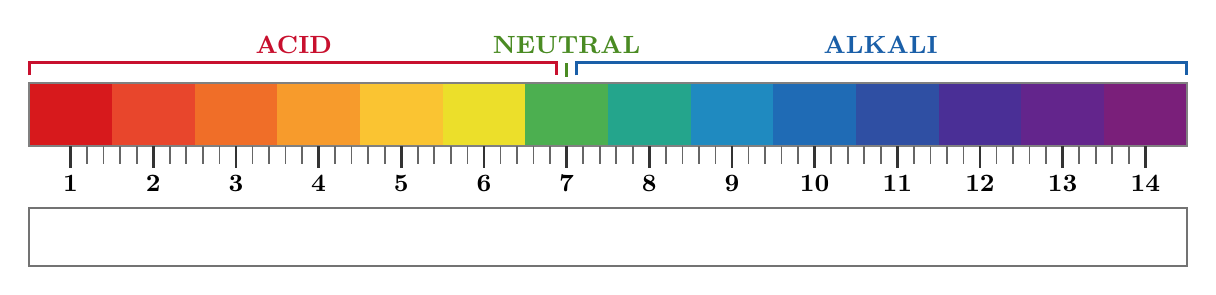
\begin{tikzpicture}[x=1.05cm, y=1cm, line width=0.8pt]

  % -- the coloured band: pH n is the CENTRE of its colour ----------------
  \foreach \n/\cc in {1/pHa, 2/pHb, 3/pHc, 4/pHd, 5/pHe, 6/pHf, 7/pHg,
                      8/pHh, 9/pHi, 10/pHj, 11/pHk, 12/pHl, 13/pHm, 14/pHn}{
    \fill[\cc] (\n-0.5,1.42) rectangle (\n+0.5,2.22);}
  \draw[black!50, line width=0.8pt] (0.5,1.42) rectangle (14.5,2.22);

  % -- the ruler: a small line every 0.2, a long numbered one at every pH --
  \foreach \k in {0,1,...,65}{
    \draw[black!60, line width=0.6pt] ({1+0.2*\k},1.42) -- ({1+0.2*\k},1.20);}
  \foreach \n in {1,...,14}{
    \draw[black!80, line width=1.0pt] (\n,1.42) -- (\n,1.14);
    \node[anchor=north, inner sep=1.5pt, font=\small\bfseries] at (\n,1.12) {\n};}

  % -- the strip the letters are written in -------------------------------
  \draw[black!55, line width=0.8pt, fill=white] (0.5,-0.10) rectangle (14.5,0.64);

  % -- the three zones. Acid is below 7 and alkali above it, so the borders
  %    fall ON 7 rather than between two cells.
  \draw[cbred, line width=1.1pt]  (0.5,2.32) -- (0.5,2.48) -- (6.88,2.48) -- (6.88,2.32);
  \draw[cbblue, line width=1.1pt] (7.12,2.32) -- (7.12,2.48) -- (14.5,2.48) -- (14.5,2.32);
  \draw[cbgreen, line width=1.3pt] (7,2.30) -- (7,2.48);
  \node[above, font=\bfseries\small, text=cbred]   at (3.7,2.46)  {ACID};
  \node[above, font=\bfseries\small, text=cbgreen] at (7.0,2.46)  {NEUTRAL};
  \node[above, font=\bfseries\small, text=cbblue]  at (10.8,2.46) {ALKALI};

\end{tikzpicture}
\end{center}

\vspace{3pt}
\noindent \textbf{(a)} Every pH below is a \textbf{decimal}. \textbf{Draw a line} on the
scale where it goes and \textbf{write the letter} in the white strip --- there are
\textbf{five small spaces} between each pair of numbers.
\textbf{(b)} Finish the last column.

\vspace{4pt}
\noindent
\begin{tabularx}{\textwidth}{|c|p{2.5cm}|c|L|c|p{2.5cm}|c|L|}
  \hline
  & \textbf{Liquid} & \textbf{pH} & \textbf{Acid, neutral} \newline \textbf{or alkali?} &
  & \textbf{Liquid} & \textbf{pH} & \textbf{Acid, neutral} \newline \textbf{or alkali?} \\
  \hline
  \textbf{A} \rule[-0.6em]{0pt}{1.9em} & lemon juice   & 2.4 & &
  \textbf{E} \rule[-0.6em]{0pt}{1.9em} & sea water     & 8.2 & \\ \hline
  \textbf{B} \rule[-0.6em]{0pt}{1.9em} & orange juice  & 3.8 & &
  \textbf{F} \rule[-0.6em]{0pt}{1.9em} & baking soda   & 9.6 & \\ \hline
  \textbf{C} \rule[-0.6em]{0pt}{1.9em} & black coffee  & 5.2 & &
  \textbf{G} \rule[-0.6em]{0pt}{1.9em} & soap          & 10.8 & \\ \hline
  \textbf{D} \rule[-0.6em]{0pt}{1.9em} & pure water    & 7.0 & &
  \textbf{H} \rule[-0.6em]{0pt}{1.9em} & bleach        & 12.6 & \\ \hline
\end{tabularx}

% -- A2 ---------------------------------------------------------------------
\qhead{A2}{Why the school buys both}

\noindent Litmus is cheap. Universal indicator costs more. Mr Bowen buys both.

\begin{remember}[Two colours, or a number]
  \key{Litmus} has \key{two} colours only: red in an acid, blue in an alkali.
  \key{Universal indicator} gives a \key{different colour for every pH number},
  so it gives you a number instead of just a word.
\end{remember}

\vspace{2pt}
\noindent Mr Bowen tests two liquids with \textbf{red litmus paper}. Both turn it blue.
One is pH 8 and the other is pH 13. Explain why litmus \textbf{cannot} tell him which is
which, and say which indicator he should use instead.

Start: \eng{``Litmus can only show\ldots''} then
\eng{``\ldots because both liquids are\ldots''}

\qlines{3}

% -- A3 ---------------------------------------------------------------------
\qhead{A3}{The end that nobody worries about}

\noindent A student says: \emph{``Acids are the dangerous ones. pH 13 is safe, because
13 is a big number.''}

\vspace{4pt}
\noindent Mr Bowen keeps a bottle of oven cleaner under his kitchen sink. Its pH is
\textbf{13}. Explain why the student is wrong. Use the word \eng{corrosive}.
\qlines{3}

% -- A4 ---------------------------------------------------------------------
% Atomic-ish block, and the last question of the section, so the tick table and
% the sentences cannot strand a heading.
\qhead{A4}{Neutralisation}

\begin{remember}[What neutralisation does]
  Add a \key{base} to an \key{acid} and they cancel each other out. The acid
  \key{stops being an acid} --- the pH moves \key{towards 7}.
\end{remember}

\noindent \textbf{(a)} Mr Bowen's garden soil has a pH of \textbf{4}, and rice will not
grow in it. He must move the pH \textbf{up} to about 7. Tick the \textbf{one} thing he
should dig into the soil.

\vspace{4pt}
\noindent
\begin{tabularx}{\textwidth}{|L|c|L|c|}
  \hline
  \textbf{What he could add} & \textbf{Tick one} & \textbf{What he could add} &
  \textbf{Tick one} \\
  \hline
  vinegar, pH 3 \rule[-0.6em]{0pt}{1.9em} & &
  lime powder, pH 12 \rule[-0.6em]{0pt}{1.9em} & \\ \hline
  lemon juice, pH 2 \rule[-0.6em]{0pt}{1.9em} & &
  pure water, pH 7 \rule[-0.6em]{0pt}{1.9em} & \\ \hline
\end{tabularx}

\vspace{7pt}
\noindent \textbf{(b)} Explain your choice in full sentences. Say what happens to the
pH of the soil.
\qlines{3}

% ===========================================================================
% SECTION B -- SCIENCE 2.7
% ===========================================================================
\hwsection{Section B \textperiodcentered\ Science 2.7 --- Compounds and Mixtures}

% -- B1 ---------------------------------------------------------------------
\qhead{B1}{Compound or mixture?}

\noindent Tick one box in each row.

\begin{remember}[The test is whether you can get it back]
  A \key{mixture} is stirred together, so you can \key{separate} it again --- with a
  magnet, a filter, or by boiling. A \key{compound} is \key{bonded} together: it is a
  \key{new substance}, and a magnet will not undo it.
\end{remember}

\vspace{2pt}
\noindent
\begin{tabularx}{\textwidth}{|L|c|c|L|c|c|}
  \hline
  & \textbf{Compound} & \textbf{Mixture} & & \textbf{Compound} & \textbf{Mixture} \\
  \hline
  air \rule[-0.6em]{0pt}{1.9em}                & & &
  water, \ch{H_2O} \rule[-0.6em]{0pt}{1.9em}   & & \\ \hline
  salt, \ch{NaCl} \rule[-0.6em]{0pt}{1.9em}    & & &
  sea water \rule[-0.6em]{0pt}{1.9em}          & & \\ \hline
  sand stirred into salt \rule[-0.6em]{0pt}{1.9em} & & &
  carbon dioxide, \ch{CO_2} \rule[-0.6em]{0pt}{1.9em} & & \\ \hline
  mineral water \rule[-0.6em]{0pt}{1.9em}      & & &
  iron sulfide, \ch{FeS} \rule[-0.6em]{0pt}{1.9em} & & \\ \hline
\end{tabularx}

% -- B2 ---------------------------------------------------------------------
\qhead{B2}{Iron and sulfur, twice}

\noindent Mr Bowen puts iron filings and yellow sulfur powder in a dish and
\textbf{stirs} them. Then he puts a second lot in a test tube and \textbf{heats} it
until it glows.

\vspace{5pt}
\noindent He holds a magnet over each one. The magnet pulls the iron out of the
\textbf{first} dish. It does nothing at all to the \textbf{second}.

\vspace{5pt}
\noindent Explain, in full sentences, what heating did and why the magnet stopped
working. Start: \eng{``Before it was heated, the iron and the sulfur were\ldots''}
then \eng{``Heating made the atoms\ldots''}

\qlines{3}

% ===========================================================================
% SECTION C -- MATHEMATICS 2.6
% ===========================================================================
\hwsection{Section C \textperiodcentered\ Mathematics 2.6 --- Inequalities}

% -- C1 ---------------------------------------------------------------------
\qhead{C1}{Say it in English}

\noindent Write $<$ or $>$ in each box, then write the whole thing as an English
sentence. The first one is done for you.

\begin{wordhelp}[Word help --- the words a question uses instead of the signs]
  \begin{tabularx}{\linewidth}{@{}l@{\hspace{16pt}}X@{}}
    \eng{is less than} \sep $<$ & also \textbf{fewer than}, \textbf{below},
      \textbf{under}. \emph{Under 18} means age $<$ 18 \\
    \eng{is greater than} \sep $>$ & also \textbf{more than}, \textbf{above},
      \textbf{over}. \eng{Greater} is not \eng{great} \\
  \end{tabularx}
\end{wordhelp}

\vspace{2pt}
\noindent
% A number after \nbox must be braced. \nbox sets an \fbox, which is an Ord
% atom, so a bare "-3" after it is read as a BINARY minus and prints as
% "- 3" with a gap. {-3} keeps the sign on the numeral.
\begin{tabularx}{\textwidth}{|c|c|L|}
  \hline
  \textbf{The numbers} & \textbf{$<$ or $>$} & \textbf{Say it in English} \\
  \hline
  $6 \;\nbox\; 11$ \rule[-0.6em]{0pt}{1.9em}    & $<$ & 6 is less than 11 \\ \hline
  $9 \;\nbox\; 2$ \rule[-0.6em]{0pt}{1.9em}     & & \\ \hline
  $-4 \;\nbox\; {1}$ \rule[-0.6em]{0pt}{1.9em}  & & \\ \hline
  $-7 \;\nbox\; {-3}$ \rule[-0.6em]{0pt}{1.9em} & & \\ \hline
\end{tabularx}

% -- C2 ---------------------------------------------------------------------
% THE CROSSOVER. Section A's eleven liquids, read with < and >. It is reprinted
% here rather than left as "look back at A1" because A1 is three pages earlier
% and a student who cannot find it stops working.
\qhead{C2}{Which liquids does the inequality mean?}

\noindent Here are the eight liquids from \textbf{A1} again, with their pH.

\vspace{4pt}
\begin{center}
\footnotesize
\renewcommand{\arraystretch}{1.15}%
% 11 columns: at the default 6pt of \tabcolsep each side this is 18.2 cm and
% hangs 1.2 cm past the right margin.
\setlength{\tabcolsep}{3pt}%
\begin{tabular}{|*{8}{>{\centering\arraybackslash}p{1.68cm}|}}
  \hline
  \textbf{A} & \textbf{B} & \textbf{C} & \textbf{D} &
  \textbf{E} & \textbf{F} & \textbf{G} & \textbf{H} \\
  \hline
  lemon juice & orange juice & black coffee & pure water &
  sea water & baking soda & soap & bleach \\
  \hline
  \textbf{2.4} & \textbf{3.8} & \textbf{5.2} & \textbf{7.0} &
  \textbf{8.2} & \textbf{9.6} & \textbf{10.8} & \textbf{12.6} \\
  \hline
\end{tabular}
\renewcommand{\arraystretch}{1.45}%
\end{center}

\vspace{6pt}
\noindent The letter $p$ stands for the pH of a liquid. For each inequality, write the
letters of \textbf{every} liquid that works.

\begin{remember}[The number in the inequality never works itself]
  $p > 9.6$ means \key{greater than} 9.6. A liquid at \key{exactly} 9.6 does
  \key{not} count. \; This is the open circle: the circle is empty because that
  number is left out.
\end{remember}

\vspace{2pt}
\noindent One of the six has \textbf{no answer at all}. If you find it, write
\textbf{none}.

\vspace{6pt}
\begin{enumerate}[label=(\alph*), itemsep=9pt]
  \item $p < 7$ \hfill \blank[11.0cm]
  \item $p > 7$ \hfill \blank[11.0cm]
  \item $p > 9.6$ \hfill \blank[11.0cm]
  \item $p < 3.8$ \hfill \blank[11.0cm]
  \item $p > 5$ \textbf{and} $p < 9$ \hfill \blank[11.0cm]
  \item $p > 12.6$ \hfill \blank[11.0cm]
\end{enumerate}

% -- C3 ---------------------------------------------------------------------
\qhead{C3}{Now write the inequality}

\noindent Each sentence is a real rule. Write it using $<$ or $>$. Use the letter
given.

\vspace{2pt}
\begin{enumerate}[label=(\alph*), itemsep=10pt]
  \item A swimming pool is safe when its pH is \textbf{above} 7.2. \; Use $p$.
        \hfill \blank[4.4cm]
  \item Rain is called acid rain when its pH is \textbf{below} 5.6. \; Use $r$.
        \hfill \blank[4.4cm]
  \item Rice grows when the soil pH is \textbf{more than} 5. \; Use $s$.
        \hfill \blank[4.4cm]
  \item A lab liquid is corrosive when its pH is \textbf{under} 2 \textbf{or}
        \textbf{over} 12. \; Use $c$. Write \textbf{two} inequalities.
        \ansline[7.2cm]
\end{enumerate}

% -- C4 ---------------------------------------------------------------------
\qhead{C4}{Read the line, then draw the line}

\noindent \textbf{(a)} Write the inequality each number line shows. Use $x$.

\vspace{7pt}
\noindent
\begin{minipage}[c]{0.62\textwidth}\numlinemark{-1}{7}{5}{-1.6}\end{minipage}%
\begin{minipage}[c]{0.36\textwidth}(i) \; \blank[3.4cm]\end{minipage}

\vspace{9pt}
\noindent
\begin{minipage}[c]{0.62\textwidth}\numlinemark{-5}{3}{-3}{3.6}\end{minipage}%
\begin{minipage}[c]{0.36\textwidth}(ii) \; \blank[3.4cm]\end{minipage}

\vspace{10pt}
\noindent \textbf{(b)} Now draw this one. Open circle, then an arrow.

\vspace{7pt}
\noindent
\begin{minipage}[c]{0.62\textwidth}\numline{-5}{3}\end{minipage}%
\begin{minipage}[c]{0.36\textwidth}$m > -2$\end{minipage}



% -- C5 ---------------------------------------------------------------------
\qhead{C5}{The smallest one that works}

\noindent An \eng{integer} is a whole number: negative, zero or positive.

\vspace{2pt}
\begin{multicols}{2}
\begin{enumerate}[label=(\alph*), itemsep=10pt]
  \item $x > 6$. Smallest integer? \blank[1.8cm]
  \item $y < -4$. Largest integer? \blank[1.8cm]
  \item $n > -1$. Smallest integer? \blank[1.8cm]
  \item $t > 2.5$. Smallest integer? \blank[1.8cm]
\end{enumerate}
\end{multicols}

% ===========================================================================
% SECTION D -- MATHEMATICS 2.5
% ===========================================================================
\hwsection{Section D \textperiodcentered\ Mathematics 2.5 --- Equations and Formulae}

% -- D1 ---------------------------------------------------------------------
\qhead{D1}{Put it back in and see}

\noindent Someone has already written an answer. Put it back into the equation. Tick
\textbf{right} or \textbf{wrong}, and if it is wrong, write the correct answer.

\begin{remember}[Checking is one line of work]
  To check $x - 7 = 5$ when somebody says $x = 2$, \key{put 2 in}: \;
  $2 - 7 = -5$, not 5. So it is wrong.
\end{remember}

\vspace{2pt}
\noindent
\begin{tabularx}{\textwidth}{|p{3.0cm}|p{2.6cm}|c|c|L|}
  \hline
  \textbf{Equation} & \textbf{Their answer} & \textbf{Right} & \textbf{Wrong} &
  \textbf{If wrong, write it} \\
  \hline
  $x - 7 = 5$ \rule[-0.6em]{0pt}{1.9em}  & $x = 2$  & & & \\ \hline
  $3y = 24$ \rule[-0.6em]{0pt}{1.9em}    & $y = 8$  & & & \\ \hline
  $m + 9 = 15$ \rule[-0.6em]{0pt}{1.9em} & $m = 24$ & & & \\ \hline
  $k - 6 = 10$ \rule[-0.6em]{0pt}{1.9em} & $k = 4$  & & & \\ \hline
\end{tabularx}

% -- D2 ---------------------------------------------------------------------
% There was a block of six bare ONE-STEP equations here -- x + 8 = 23, 7m = 56,
% n / 4 = 9, and two written the other way round. It came out for the page
% target and it is the right one to lose: D3(a), (c) and (d) are one-step
% equations arrived at from a formula, which is the same solving with a reason
% attached, and D1 already gives the section its easy way in. The only thing
% that left with it is the equation written backwards, 31 = t + 16, and that
% now appears nowhere on the packet -- say it out loud when you hand this back.
\qhead{D2}{Two steps}

\noindent Undo the \textbf{last} step first. Write the middle line.

\begin{remember}[Last on, first off]
  $2a + 4 = 18$. The last thing done to $a$ was \key{add 4}, so undo that first.

  \smallskip
  \hspace*{1.2em}$18 - 4 = 14$, \; then $14 \div 2 = \mathbf{7}$. \quad
  Check: $2 \times 7 + 4 = 18$. \;
  {\color{cbred}\bfseries Not $18 \div 2$ first.}
\end{remember}

\vspace{2pt}
\begin{multicols}{2}
\begin{enumerate}[label=(\alph*), itemsep=11pt]
  \item $3a + 5 = 26$ \hfill $a = \blank[1.8cm]$
  \item $4b - 7 = 25$ \hfill $b = \blank[1.8cm]$
  \item $5c + 12 = 47$ \hfill $c = \blank[1.8cm]$
  \item $2d - 9 = 15$ \hfill $d = \blank[1.8cm]$
  \item $6m + 4 = 40$ \hfill $m = \blank[1.8cm]$
  \item $8n - 3 = 45$ \hfill $n = \blank[1.8cm]$
\end{enumerate}
\end{multicols}

% -- D3 ---------------------------------------------------------------------
% The question the whole section is for: a formula from 2.2 turned into an
% equation by 2.5. Part (e) is the formula the graph in F3 is drawn from.
\qhead{D3}{You are given the formula. Find the letter.}

\noindent In each one you are told the \textbf{answer} the formula gives. Work
backwards to find the letter. \textbf{Write the equation first.}

\begin{remember}[Two jobs, in this order]
  A taxi costs \; \expr{C = 15n + 20} \; where $n$ is the number of kilometres.
  Mr Bowen's taxi cost \textbf{95}. How far did he go?

  \medskip
  \hspace*{1.2em}\textbf{1. Put the number in:} \quad $15n + 20 = 95$

  \smallskip
  \hspace*{1.2em}\textbf{2. Solve it:} \quad $95 - 20 = 75$, \; then
  $75 \div 15 = \mathbf{5}$. \quad He went 5 km.
\end{remember}

\vspace{2pt}
\begin{enumerate}[label=(\alph*), itemsep=10pt]
  \item $P = 4s$ \; (perimeter of a square, side $s$). \; $P = 52$.
        \hfill $s = \blank[2.2cm]$
  \item $C = 8n + 15$ \; (cost of $n$ tickets). \; $C = 95$.
        \hfill $n = \blank[2.2cm]$
  \item $d = 60t$ \; (km travelled in $t$ hours). \; $d = 480$.
        \hfill $t = \blank[2.2cm]$
  \item $V = 30h$ \; (\ccm\ in a tank at depth $h$ cm). \; $V = 420$.
        \hfill $h = \blank[2.2cm]$
  \item $m = 60 + v$ \; (grams: a beaker plus $v$ \ccm\ of water). \; $m = 145$.
        \hfill $v = \blank[2.2cm]$
  \item $F = 2n - 6$. \; $F = 38$.
        \hfill $n = \blank[2.2cm]$
\end{enumerate}

% -- D4 ---------------------------------------------------------------------
\qhead{D4}{Word problems}

\noindent Write the equation, then solve it. Show your working in the box.

\vspace{4pt}
\noindent \textbf{(a)} Mr Bowen's jug holds \textbf{340} \ccm\ of water. He pours the
\textbf{same amount} into each of \textbf{6} beakers, and \textbf{40} \ccm\ is left in
the jug. How much water went into each beaker?

\begin{workspace}[2.3cm]\end{workspace}

\noindent \textbf{(b)} Mr Bowen has some fish. He buys \textbf{4} more. Then his cat
eats \textbf{half} of all of them. He now has \textbf{6} fish. How many did he have at
the start?

\begin{workspace}[2.3cm]\end{workspace}

% ===========================================================================
% SECTION E -- MATHEMATICS 3.1 AND 3.2
% ===========================================================================
\hwsection{Section E \textperiodcentered\ Mathematics 3.1--3.2 --- Place Value and Rounding}

% -- E1 ---------------------------------------------------------------------
\qhead{E1}{Move the digits}

\noindent No calculator.

\begin{remember}[The point never moves --- the digits do]
  $7.2 \times 10^3$ is \key{7200}. \; {\color{cbred}\bfseries Not 7.2000.} \\
  Multiplying moves the digits \key{left}. Dividing moves them \key{right}. The
  power counts \key{how many places}.
\end{remember}

\vspace{2pt}
\begin{multicols}{3}
\begin{enumerate}[label=(\alph*), itemsep=10pt]
  \item $3.7 \times 100 = \blank[1.7cm]$
  \item $4.5 \times 10^3 = \blank[1.7cm]$
  \item $26 \times 10^4 = \blank[1.7cm]$
  \item $940 \div 100 = \blank[1.7cm]$
  \item $63 \div 10^3 = \blank[1.7cm]$
  \item $5 \div 10^4 = \blank[1.7cm]$
\end{enumerate}
\end{multicols}

% -- E2 ---------------------------------------------------------------------
% There was a mass-ladder question here -- 3 kg to g, 250 mg to g, 1.8 t to kg,
% 6 kg to mg. It came out for the page target. It is the only cut on this
% packet that loses a stated objective of its section, so it does not simply
% disappear: the extra sheet, hw08x, teaches the ladder at length in Part 4,
% and every student gets that sheet. Set it alongside this packet, not instead.
\qhead{E2}{Round it}

\begin{remember}[Keep the zero]
  $34.9892$ to \key{1 decimal place} is \key{35.0}, not 35. The $.0$ is what shows
  you rounded to one place. Writing 35 loses the mark.
\end{remember}

% One table, not two headed multicols blocks. As two blocks the E3 heading and
% its orange box were about 5 cm and stranded the heading alone at the foot of
% a page; the table is also less of the page for the same eight numbers.
\vspace{2pt}
\noindent
\begin{tabularx}{\textwidth}{|>{\raggedright\arraybackslash}p{3.5cm}|X|X|X|X|}
  \hline
  \textbf{To 1 decimal place} \rule[-0.7em]{0pt}{2.1em} &
    $7.34$ & $12.87$ & $0.952$ & $29.96$ \\ \hline
  \rule[-0.8em]{0pt}{2.2em} & & & & \\ \hline
  \textbf{To 2 decimal places} \rule[-0.7em]{0pt}{2.1em} &
    $5.376$ & $0.0961$ & $8.2449$ & $3.997$ \\ \hline
  \rule[-0.8em]{0pt}{2.2em} & & & & \\ \hline
\end{tabularx}

% -- E3 ---------------------------------------------------------------------
\qhead{E3}{One place further}

\begin{remember}[Work out one extra digit, then round]
  For $58 \div 7$ correct to \key{3 decimal places}, divide to \key{4}: $8.2857$. The
  4th digit is 7, so it is \key{8.286}, not 8.285. \; Calculator allowed here only.
\end{remember}

\vspace{2pt}
\begin{multicols}{2}
\begin{enumerate}[label=(\alph*), itemsep=10pt]
  \item $47 \div 9$, correct to 2 d.p. \hfill \blank[2.4cm]
  \item $45 \div 7$, correct to 2 d.p. \hfill \blank[2.4cm]
  \item $26 \div 3$, correct to 3 d.p. \hfill \blank[2.4cm]
  \item $100 \div 7$, correct to 3 d.p. \hfill \blank[2.4cm]
\end{enumerate}
\end{multicols}

% -- E4 ---------------------------------------------------------------------
\qhead{E4}{Mr Bowen's homework}

\noindent One of these four is right. Find it, and correct the other three.

\vspace{4pt}
\begin{multicols}{2}
\begin{enumerate}[label=(\alph*), itemsep=10pt]
  \item $6.4 \times 10^3 = 6.4000$ \; \blank[2.4cm]
  \item $380 \div 10^2 = 38$ \; \blank[2.4cm]
  \item $2.996$ to 2 d.p. $= 2.99$ \; \blank[2.4cm]
  \item $0.83$ to 1 d.p. $= 0.8$ \; \blank[2.4cm]
\end{enumerate}
\end{multicols}

% ===========================================================================
% SECTION F -- THE BRIDGE
% ===========================================================================
\hwsection[cbgreen]{Section F \textperiodcentered\ Where it all meets --- reading a scale}

\noindent In \textbf{A1} you were given a number and had to find the place. Here it is
the other way round: you are given the place and have to find the number. A cylinder is
a number line stood on its end, and a graph has two --- and both of them ask the same
question first: \textbf{how much is one small line worth?}

% -- F1 ---------------------------------------------------------------------
\qhead[cbgreen]{F1}{How much is one small line worth?}

\begin{remember}[Count the spaces, not the lines]
  Look at \key{two numbered lines}. Count the \key{spaces} between them --- the gaps,
  not the marks. Then \key{divide}. \; From \textbf{0} to \textbf{10} with \textbf{5}
  spaces: \; $10 \div 5 = \mathbf{2}$, \; so one small line is \key{worth} 2.

  \smallskip
  \eng{A scale} is the row of lines and numbers on an instrument. \eng{Scales} is the
  machine you stand on to find your mass --- a different word.
\end{remember}

\vspace{2pt}
\noindent
\begin{tabularx}{\textwidth}{|c|c|c|L|}
  \hline
  \textbf{From} & \textbf{To} & \textbf{Spaces between them} &
  \textbf{One small line is worth} \\
  \hline
  0 \rule[-0.6em]{0pt}{1.9em}   & 10  & 5  & \textbf{2} \\ \hline
  0 \rule[-0.6em]{0pt}{1.9em}   & 1   & 10 & \\ \hline
  20 \rule[-0.6em]{0pt}{1.9em}  & 30  & 4  & \\ \hline
  0 \rule[-0.6em]{0pt}{1.9em}   & 5   & 10 & \\ \hline
  50 \rule[-0.6em]{0pt}{1.9em}  & 100 & 5  & \\ \hline
\end{tabularx}

% -- F2 ---------------------------------------------------------------------
% Atomic block: a tikzpicture cannot be broken, so the four cylinders and their
% answer table sit together at the top of their own page.
\qhead[cbgreen]{F2}{Four measuring cylinders}

\noindent Same small lines on all four; only the \textbf{numbers} differ. Read the
bottom of the meniscus.

\vspace{6pt}
\begin{center}
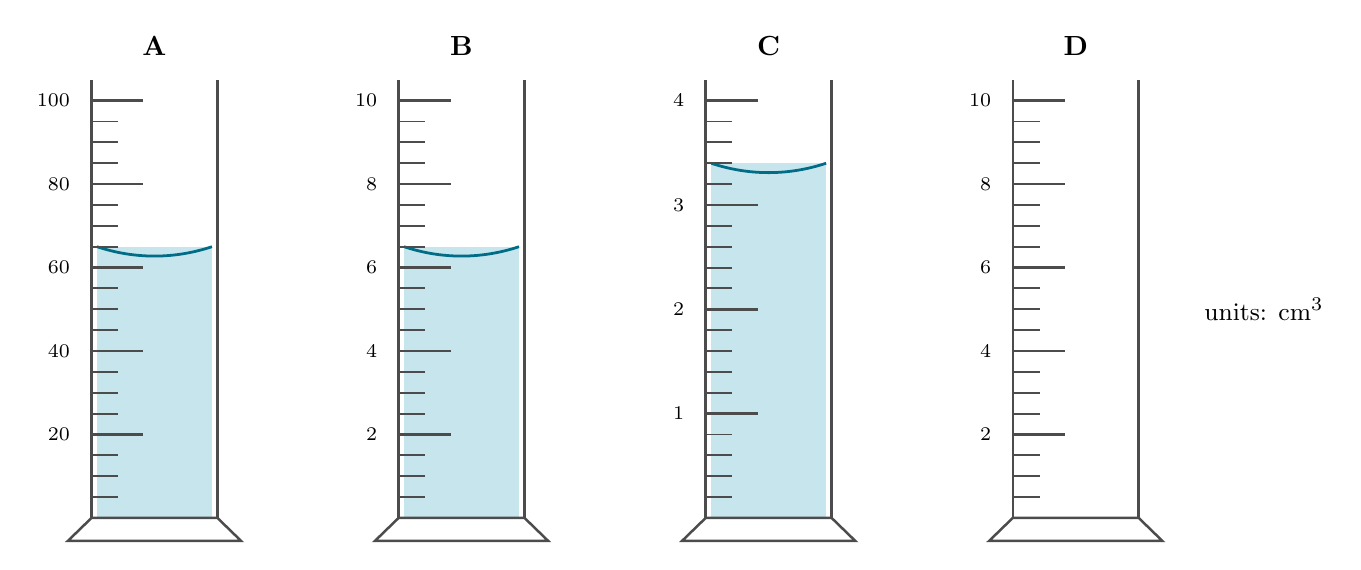
\begin{tikzpicture}[x=1cm, y=0.265cm, line width=0.9pt]
  \cyl{0}{A}{4/20, 8/40, 12/60, 16/80, 20/100}{13}
  \cyl{3.9}{B}{4/2, 8/4, 12/6, 16/8, 20/10}{13}
  \cyl{7.8}{C}{5/1, 10/2, 15/3, 20/4}{17}
  \cyl{11.7}{D}{4/2, 8/4, 12/6, 16/8, 20/10}{0}
  \node[anchor=west, font=\small] at (14.0,10) {units: \ccm};
\end{tikzpicture}
\end{center}

\vspace{4pt}
\noindent
\begin{tabularx}{\textwidth}{|c|L|L|}
  \hline
  & \textbf{One small line is worth} & \textbf{The volume of water is} \\
  \hline
  \textbf{A} \rule[-0.7em]{0pt}{2.1em} & & \\ \hline
  \textbf{B} \rule[-0.7em]{0pt}{2.1em} & & \\ \hline
  \textbf{C} \rule[-0.7em]{0pt}{2.1em} & & \\ \hline
  \textbf{D} \rule[-0.7em]{0pt}{2.1em} & &
    \textbf{Draw} the water at $8.5$ \ccm \\ \hline
\end{tabularx}

\vspace{8pt}
\noindent \textbf{(b)} \textbf{A} and \textbf{B} are the same picture, and the water is
at the same height. Explain why the two answers are not the same number.
\qlines{2}

% -- F3 ---------------------------------------------------------------------
% Atomic block, and the last question on the packet: the graph and its
% questions cannot be split. (f) is D3(e) arrived at from the other end.
\qhead[cbgreen]{F3}{The same question, on a graph}

\noindent Mr Bowen puts an \textbf{empty} beaker on a balance, then pours water in a
little at a time and writes down the mass.

\vspace{4pt}
\begin{center}
% The grid is the question, so it is drawn big enough to count. x and y are
% scaled separately: the axes run 0-100 and 0-200 in their own units and a
% small square has to stay a square you can see across the room.
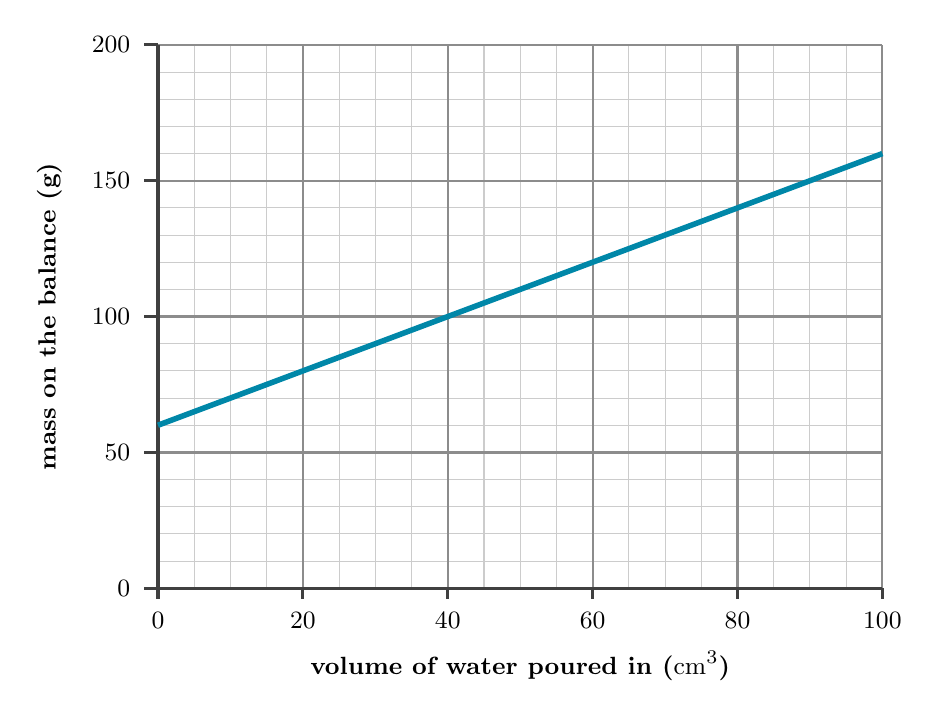
\begin{tikzpicture}[x=0.092cm, y=0.0345cm, line width=0.9pt]

  % -- graph paper: a light line at every small division -------------------
  \draw[black!20, line width=0.4pt] (0,0) grid[xstep=5, ystep=10] (100,200);
  \draw[black!45, line width=0.8pt] (0,0) grid[xstep=20, ystep=50] (100,200);

  % -- axes ----------------------------------------------------------------
  \draw[black!75, line width=1.2pt] (0,0) -- (0,200);
  \draw[black!75, line width=1.2pt] (0,0) -- (100,0);

  % -- numbered lines only; the small ones are deliberately not numbered ---
  \foreach \v in {0,20,40,60,80,100}{
    \draw[black!75, line width=1.1pt] (\v,0) -- (\v,-4);
    \node[below=1pt, font=\small] at (\v,-4) {\v};}
  \foreach \v in {0,50,100,150,200}{
    \draw[black!75, line width=1.1pt] (0,\v) -- (-2,\v);
    \node[left=1pt, font=\small] at (-2,\v) {\v};}

  % -- the line: mass = 60 + volume ---------------------------------------
  \draw[cbteal, line width=2.0pt] (0,60) -- (100,160);

  % -- axis titles ---------------------------------------------------------
  \node[below=15pt, font=\small\bfseries] at (50,-4) {volume of water poured in (\ccm)};
  \node[rotate=90, font=\small\bfseries] at (-15,100) {mass on the balance (g)};

\end{tikzpicture}
\end{center}

\vspace{4pt}
\begin{enumerate}[label=(\alph*), itemsep=8pt]
  \item How much is one small line worth on the \textbf{across} axis?
        \hfill \blank[3.2cm]
  \item How much is one small line worth on the \textbf{up} axis?
        \hfill \blank[3.2cm]
  \item What is the mass when \textbf{40} \ccm\ has been poured in?
        \hfill \blank[3.2cm]
  \item The balance reads \textbf{130} g. How much water is in the beaker?
        \hfill \blank[3.2cm]
  \item What is the mass of the \textbf{empty} beaker? Say how you know.
        \ansline[9.6cm]
        \ansline[9.6cm]
  \item Write a \textbf{formula} for the mass $m$ grams when $v$ \ccm\ of water has
        been poured in. \ansfor[4.0cm]{m}
\end{enumerate}

% ===========================================================================
% ANSWER KEY -- TEACHER COPY ONLY
% ===========================================================================
\ifkey
\clearpage

\hwsection[cbred]{Answer Key --- Teacher Copy}

\linespread{1.0}\selectfont
\setlist[enumerate]{itemsep=2pt, topsep=3pt, leftmargin=*}
\setlist[itemize]{itemsep=2pt, topsep=3pt, leftmargin=*}

\qhead[cbred]{A1}{Put each liquid on the scale}
\noindent One small space is \textbf{0.2}, so every pH on the list lands exactly on a
small line. Counting from the numbered line on its left: \\
\textbf{A} 2.4 --- 2 lines past 2 \sep \textbf{B} 3.8 --- 4 lines past 3 \sep
\textbf{C} 5.2 --- 1 line past 5 \sep \textbf{D} 7.0 --- \emph{on} the 7 \\
\textbf{E} 8.2 --- 1 line past 8 \sep \textbf{F} 9.6 --- 3 lines past 9 \sep
\textbf{G} 10.8 --- 4 lines past 10 \sep \textbf{H} 12.6 --- 3 lines past 12

\smallskip
\noindent Last column: A, B, C \textbf{acid} \sep D \textbf{neutral} \sep
E, F, G, H \textbf{alkali}.

\smallskip
\noindent{\small \textbf{Mark the position, not the letter.} A line within half a small
space of the right place is right; a line on the wrong side of a numbered line is not.
The error to look for is a student putting \textbf{B} at 3.8 by counting 8 small lines
instead of 4 --- they have read the 8 as eight spaces rather than eight tenths. Five
spaces to a whole number means each one is two tenths, and that is the only arithmetic
in the question. \\
\textbf{G, 10.8} is the one most often put past 11. Counting 8 lines from 10 lands at
11.6. Same error as B, one column further left. \\
\textbf{D, pure water at 7.0} is the row that separates the class, and the decimal is
why it is written 7.0 rather than 7. It is not ``a bit of both'' and it is not ``nearly
acid''; it is \textbf{exactly} 7 and the word is \textbf{neutral}. Ask for that word
specifically, and keep the answer to hand --- C2(a) and C2(b) both turn on it. \\
\textbf{E, sea water at 8.2} surprises them every year. The sea is slightly alkaline. \\
If a student writes \emph{base} instead of \emph{alkali} in the last column, correct it
now: these liquids are all dissolved in water, so the exam word is \textbf{alkali}.}

\qhead[cbred]{A2}{Why the school buys both}
\noindent Litmus has only two colours. pH 8 and pH 13 are \emph{both} alkaline, so both
turn red litmus blue, and there is no third colour for litmus to tell them apart with.
He should use \textbf{universal indicator}, because it gives a different colour for every
pH number, so it gives a number rather than just the word \emph{alkali}.

\smallskip
\noindent{\small This is the question that finds out who understood what an indicator
\emph{is}. The wrong answer to look for is ``because 13 is stronger'' --- true, but it
does not answer the question, which is about what litmus can \emph{show}. Push for the
words \textbf{two colours}. \\
A full-sentence answer is the requirement. ``Litmus only has 2 colours'' is the idea but
not the sentence; the starters are printed for a reason.}

\qhead[cbred]{A3}{The end that nobody worries about}
\noindent Wrong. A strong alkali is \textbf{corrosive} in exactly the way a strong acid
is: it attacks skin, eyes and clothes. pH 13 is as far from neutral as pH 1 is. Danger
is at \textbf{both ends} of the scale, not just the left-hand end.

\smallskip
\noindent{\small This is the misconception of Science 2.8, and it was the class vote in
the lesson --- the majority chose pH 1. Expect the same split here. \\
The detail that makes it land is that the oven cleaner is \textbf{under his kitchen
sink}, not in a lab. Students think of danger as a laboratory thing. Ask whose house has
one. \\
Accept any answer that says both ends are dangerous \emph{and} uses \emph{corrosive}
correctly. Do not accept ``13 is a big number so it is strong'' on its own --- that is
the student agreeing with the wrong sentence for a different reason.}

\qhead[cbred]{A4}{Neutralisation}
\noindent \textbf{(a)} \textbf{Lime powder, pH 12.} \\
\textbf{(b)} The soil is an acid at pH 4. Lime powder is a base, so adding it
neutralises the acid and the pH rises towards 7.

\smallskip
\noindent{\small \textbf{Pure water, pH 7} is the wrong answer worth discussing rather
than marking. It is neutral, so students reason that adding a neutral thing makes the
soil neutral. It does not --- it dilutes it and the soil is still an acid. That is a
genuinely good piece of thinking arriving at a wrong answer; say so before correcting
it. \\
Vinegar and lemon juice are acids being added to an acid, which moves the pH the wrong
way. A student who ticks one of those has not read \emph{up to about 7}. \\
In (b) the phrase to insist on is \textbf{towards 7}. ``It makes the pH bigger'' is
half the idea; neutralisation has a destination.}

\qhead[cbred]{B1}{Compound or mixture?}
\noindent \textbf{Mixtures:} air \sep sand stirred into salt \sep mineral water \sep
sea water. \\
\textbf{Compounds:} salt \ch{NaCl} \sep water \ch{H_2O} \sep carbon dioxide \ch{CO_2}
\sep iron sulfide \ch{FeS}.

\smallskip
\noindent{\small \textbf{Water and sea water on the same row is the whole question.}
\ch{H_2O} is a compound; sea water is that compound with salt and other things stirred
into it. Students who tick the same box for both have matched on the word
\emph{water}. \\
\textbf{Air} is the one they most often call a compound, because it is invisible and
feels like one substance. Ask what you can take out of it --- oxygen, for a hospital
cylinder. \\
\textbf{Mineral water} is the easy one once air has been settled, and it is on the
packet as the reward for getting air right.}

\qhead[cbred]{B2}{Iron and sulfur, twice}
\noindent Stirred, the iron and the sulfur are a \textbf{mixture}: the atoms have not
joined, so the iron is still iron and a magnet pulls it out. Heating made the atoms
\textbf{bond} together, and what is left is a \textbf{new substance}, iron sulfide. It
is a \textbf{compound}, and it is not magnetic, because it is not iron any more.

\smallskip
\noindent{\small Mark for the word \textbf{new substance}. The near-miss answer is ``the
heat melted them together'', which is a mixture description wearing a compound's
clothes --- the student thinks the iron is still in there, just stuck. It is not. \\
The magnet is the evidence and the answer should say so. A student who explains bonding
but never mentions the magnet has answered a different question. \\
Three writing lines, because this needs three sentences: what it was, what heating did,
what it is now.}

\qhead[cbred]{C1}{Say it in English}
\noindent $9 > 2$ --- ``9 is greater than 2''. \; $-4 < 1$ --- ``$-4$ is less than
1''. \; $-7 < -3$ --- ``$-7$ is less than $-3$''.

\smallskip
\noindent{\small $-7 < -3$ is the row that goes wrong, and the error is Unit 1's, not
this unit's: 7 is bigger than 3, so the student writes $>$. Send them to the number
line, or to the thermometer --- $-7$ degrees is colder. \\
The English column is the point of the question. Accept only a full sentence with
\textbf{is}: ``$-4$ less than 1'' is not it. They have known these signs since Grade 1;
what they have never done is say them out loud in English, left to right.}

\qhead[cbred]{C2}{Which liquids does the inequality mean?}
\noindent (a) $p < 7$: \textbf{A, B, C} \quad (b) $p > 7$: \textbf{E, F, G, H} \\
(c) $p > 9.6$: \textbf{G, H} \quad (d) $p < 3.8$: \textbf{A} \\
(e) $p > 5$ and $p < 9$: \textbf{C, D, E} \quad (f) $p > 12.6$: \textbf{none}

\smallskip
\noindent{\small \textbf{Four of the six turn on a liquid whose pH is exactly the number
in the inequality, and that is why this question exists.} In (c) baking soda is 9.6 and
$9.6 > 9.6$ is false, so F is out. In (d) orange juice is 3.8, so B is out. In (f)
bleach is 12.6, so nothing on the list works \emph{at all} --- and the instruction line
warns that one of the six has no answer. A student who keeps F in (c) will keep H in
(f); mark those two together and hand them back at once. \\
In (a) and (b), notice that \textbf{D, pure water, appears in neither.} 7.0 is not less
than 7 and not greater than 7. If a student has put D in both, they have read $<$ and
$>$ as ``on the acid side'' and ``on the alkali side''. \\
(e) is the two-inequality question and the only one where a liquid must satisfy both. A
student who writes C, D, E, F has checked $p > 5$ and stopped reading --- 9.6 is not
less than 9. \\
This is also a science check: (a) is exactly the list of acids and (b) is exactly the
list of alkalis. If their A1 table disagrees with their C2 answer, one of the two is
wrong and they can find out which without you.}

\qhead[cbred]{C3}{Now write the inequality}
\noindent (a) $p > 7.2$ \quad (b) $r < 5.6$ \quad (c) $s > 5$ \quad
(d) $c < 2$ \textbf{and} $c > 12$

\smallskip
\noindent{\small The vocabulary is the question: \textbf{above} and \textbf{more than}
are both $>$; \textbf{below} and \textbf{under} are both $<$. Four different English
words, two signs. \\
(d) needs \emph{two} inequalities, and it says so. A student who writes
$2 > c > 12$ has invented something that cannot be true; do not mark it wrong so much as
ask them to read it aloud --- it says $2$ is greater than $12$. \\
The decimals in (a) and (b) are not there to be hard. They are there so that the class
sees an inequality does not need a whole number in it, which is what makes C5(d)
answerable.}

\qhead[cbred]{C4}{Read the line, then draw the line}
\noindent \textbf{(a)} (i) $x < 5$ \quad (ii) $x > -3$ \\
\textbf{(b)} (i) open circle at 4, arrow \textbf{left} \quad
(ii) open circle at $-2$, arrow \textbf{right}

\smallskip
\noindent{\small In (a) the arrow direction is the answer and the circle is where it
starts. Students who read the arrowhead's number instead of the circle's write
$x < -1$ for (i). \\
In (b), check the \textbf{circle is open}. A filled circle is a different inequality
($\leq$), which is next year, and a student drawing it here has copied a dot from
somewhere. \\
(a)(ii) crosses zero, which is the only reason it is on the packet.}

\qhead[cbred]{C5}{The smallest one that works}
\noindent (a) \textbf{7} \quad (b) \textbf{$-5$} \quad (c) \textbf{0} \quad
(d) \textbf{3}

\smallskip
\noindent{\small (b) is the negative-direction trap: \emph{largest} feels as though it
should mean \emph{to the right}, so students write $-3$. Less than means \textbf{further
left}, and the largest integer below $-4$ is the one immediately to its left. \\
(c) answers \textbf{0}, and students who think zero is not really a number leave it
blank. \\
(d) is the decimal one: the circle sits between 2 and 3, so the smallest \emph{integer}
that works is 3, not 2.5 and not 2.}

\qhead[cbred]{D1}{Put it back in and see}
\noindent $x - 7 = 5$, $x = 2$: \textbf{wrong}, $x = 12$ \sep
$3y = 24$, $y = 8$: \textbf{right} \\
$m + 9 = 15$, $m = 24$: \textbf{wrong}, $m = 6$ \sep
$k - 6 = 10$, $k = 4$: \textbf{wrong}, $k = 16$

\smallskip
\noindent{\small Every wrong answer here is the \emph{same} error: the student did the
operation they could see instead of the inverse. $2$ is $7-5$; $24$ is $15+9$; $4$ is
$10-6$. Say that out loud --- three mistakes, one habit. \\
The fix is the one line of checking the box shows. A class that substitutes can settle
its own arguments, and every workbook question in 2.5 asks them to.}

\qhead[cbred]{D2}{Two steps}
\noindent (a) $26 - 5 = 21$, $21 \div 3 = \mathbf{7}$ \quad
(b) $25 + 7 = 32$, $32 \div 4 = \mathbf{8}$ \quad
(c) $47 - 12 = 35$, $35 \div 5 = \mathbf{7}$ \\
(d) $15 + 9 = 24$, $24 \div 2 = \mathbf{12}$ \quad
(e) $40 - 4 = 36$, $36 \div 6 = \mathbf{6}$ \quad
(f) $45 + 3 = 48$, $48 \div 8 = \mathbf{6}$

\smallskip
\noindent{\small Mark the \textbf{middle line}. A student who divides first gets a
number that looks like an answer, and nothing in the final figure shows what went
wrong. \\
The dividing-first error on (a) gives $26 \div 3$, which is not a whole number --- and
that is useful. Tell them: if the first step does not divide exactly, you almost
certainly did it in the wrong order.}

\qhead[cbred]{D3}{You are given the formula. Find the letter.}
\noindent (a) $4s = 52$, $s = \mathbf{13}$ \quad
(b) $8n + 15 = 95$, $80 \div 8$, $n = \mathbf{10}$ \quad
(c) $60t = 480$, $t = \mathbf{8}$ \\
(d) $30h = 420$, $h = \mathbf{14}$ \quad
(e) $60 + v = 145$, $v = \mathbf{85}$ \quad
(f) $2n - 6 = 38$, $44 \div 2$, $n = \mathbf{22}$

\smallskip
\noindent{\small \textbf{The instruction is to write the equation first, and that is what
to mark.} A student who writes only ``13'' has probably divided 52 by 4 for good reasons,
but the packet is teaching a formula becoming an equation, and the equation is the
evidence. \\
(a), (c) and (d) are one step; (b) and (f) are two. The mixture is deliberate --- the
formula does not announce which kind it is, and deciding that is the skill. \\
\textbf{(e) is the formula the graph in F3 is drawn from.} If a student notices, that is
the best thing that will happen on this packet; F3(f) asks for it from the other end.}

\qhead[cbred]{D4}{Word problems}
\noindent \textbf{(a)} $6w + 40 = 340$; \; $340 - 40 = 300$, \; $300 \div 6 = 50$.
\textbf{50} \ccm\ in each beaker. \\
\textbf{(b)} $(f + 4) \div 2 = 6$; \; $6 \times 2 = 12$, \; $12 - 4 = 8$.
He had \textbf{8} fish.

\smallskip
\noindent{\small (a) is the one where the English decides everything. \emph{40 is left in
the jug} means 40 was never poured, so it is $+\,40$ on the beaker side, and the students
who write $6w = 340$ have skipped the clause. Make them point at the words. \\
(b) is the only question on the packet where the last operation is a division, so
\emph{undo the last step first} means multiply. Students reverse it and get
$(6 - 4) \times 2 = 4$. The check is the cure: 8 fish, buy 4, that is 12, the cat eats
half, 6 left. \\
Read (b) completely straight. Do not explain the cat.}

\qhead[cbred]{E1}{Move the digits}
\noindent (a) $370$ \quad (b) $4500$ \quad (c) $260\,000$ \quad
(d) $9.4$ \quad (e) $0.063$ \quad (f) $0.0005$

\smallskip
\noindent{\small (e) and (f) are where the zeros go missing. $63 \div 10^3$ is
\emph{three} places right: $6.3$, $0.63$, $0.063$. A student who writes $0.63$ has moved
two. \\
(f) is the extreme case --- four places from a single digit, so three zeros have to be
written before the 5 arrives. \\
(b) is the one that catches the folk rule: ``add three zeros'' gives $4.5000$, which is
just $4.5$.}

\qhead[cbred]{E2}{Round it}
\noindent \textbf{Top row, to 1 d.p.:} \; $7.3$ \sep $12.9$ \sep $\mathbf{1.0}$ \sep
$\mathbf{30.0}$ \\
\textbf{Bottom row, to 2 d.p.:} \; $5.38$ \sep $\mathbf{0.10}$ \sep $8.24$ \sep
$\mathbf{4.00}$

\smallskip
\noindent{\small \textbf{Four of the eight are the same question}, and it is the one from
the lesson: the digit carries and the trailing zero must stay. $0.952$ is $1.0$ not $1$;
$29.96$ is $30.0$ not $30$; $0.0961$ is $0.10$ not $0.1$; $3.997$ is $4.00$ not $4$. The
zero is what shows how many places you rounded to, and dropping it loses the mark even
though the number is the same size. \\
$8.2449$ is the opposite trap and the only one on the packet: the third decimal is 4, so
it rounds \emph{down} to $8.24$. Students who look at the \emph{fourth} digit, see 9,
round the 4 up to 5 and then round again get $8.25$. Rounding happens once, from the
original number.}

\qhead[cbred]{E3}{One place further}
\noindent (a) $5.2222\ldots = \mathbf{5.22}$ \quad
(b) $6.4285\ldots = \mathbf{6.43}$ \quad
(c) $8.6666\ldots = \mathbf{8.667}$ \quad
(d) $14.2857\ldots = \mathbf{14.286}$

\smallskip
\noindent{\small (b) and (d) are the ones that need the extra digit. (b) to two places
means dividing to three: $6.428$, and the 8 rounds the 2 up to 3. A student who stops at
two places sees $6.42$ and never finds out. \\
(a) and (c) are the recurring ones, and (c) is the reminder that 6 always rounds up ---
$8.6666$ to 3 d.p. is $8.667$.}

\qhead[cbred]{E4}{Mr Bowen's homework}
\noindent (a) \textbf{wrong} --- $6400$. The digits move; you do not write zeros on the
end of a decimal. \\
(b) \textbf{wrong} --- $3.8$. Two places right from $380$ is $38$, then $3.8$. \\
(c) \textbf{wrong} --- $3.00$. The 6 rounds the second 9 up, which carries all the way,
and all three digits of $3.00$ are needed. \\
(d) \textbf{right.}

\smallskip
\noindent{\small (c) is the hardest item in Section E: it is the carry \emph{and} the
trailing zeros in one number, and the answer no longer looks like the question. \\
The instruction says one of the four is right. A student who corrects all four has not
read it; a student who corrects none has decided Mr Bowen is reliable.}

\qhead[cbred]{F1}{How much is one small line worth?}
\noindent $0$ to $1$, 10 spaces: \textbf{0.1} \quad
$20$ to $30$, 4 spaces: \textbf{2.5} \quad
$0$ to $5$, 10 spaces: \textbf{0.5} \quad
$50$ to $100$, 5 spaces: \textbf{10}

\smallskip
\noindent{\small The $20$ to $30$ row is the one to watch: the gap is $10$, not $30$.
Students subtract nothing and divide 30 by 4. Say \textbf{the gap} rather than
\textbf{the numbers} when you hand this back. \\
The $0$ to $5$ row is the one that proves the answer depends on \emph{both} numbers:
the gap is bigger than the first row's and the answer is smaller, because there are twice
as many spaces. \\
Counting lines instead of spaces gives 6 spaces where there are 5, and it is the error
this whole section exists to kill. A scale from 0 to 10 in fives has \emph{six} marks and
\emph{five} gaps.}

\qhead[cbred]{F2}{Four measuring cylinders}
\noindent \textbf{A}: one line $= 5$ \ccm, water $= \mathbf{65}$ \ccm \\
\textbf{B}: one line $= 0.5$ \ccm, water $= \mathbf{6.5}$ \ccm \\
\textbf{C}: one line $= 0.2$ \ccm, water $= \mathbf{3.4}$ \ccm \\
\textbf{D}: one line $= 0.5$ \ccm; $8.5$ \ccm\ is \textbf{17 small lines up}, which is
one line above the 8.

\smallskip
\noindent \textbf{(b)} The small lines are worth different amounts. On A each line is
$5$ \ccm\ and on B each line is $0.5$ \ccm, so the same height is ten times as much on
A as on B.

\smallskip
\noindent{\small \textbf{(b) is the question, and A and B are drawn identically on
purpose.} The two answers differ by exactly a factor of ten, which is Section E standing
in a cylinder. If a student has written 65 for both, they read the picture and never read
the numbers --- which is the single commonest error in practical work. \\
\textbf{C} is the hardest read: five spaces per number, so one line is $0.2$, and 17
lines is $3.4$. Students who assume 0.5 because B was 0.5 get $8.5$. Make them count the
spaces between two numbers on \emph{that} cylinder. \\
In D, check the level is drawn one line \emph{above} the 8, not on it, and that the
meniscus dips.}

\qhead[cbred]{F3}{The same question, on a graph}
\noindent (a) $\mathbf{5}$ \ccm \quad (b) $\mathbf{10}$ g \quad
(c) $\mathbf{100}$ g \quad (d) $\mathbf{70}$ \ccm \\
(e) $\mathbf{60}$ g --- it is where the line meets the up axis, which is the mass when
no water has been poured in at all. \\
(f) $m = 60 + v$

\smallskip
\noindent{\small (a) and (b) are F1 on a graph, and they must be done before (c): four
spaces per 20 across, five spaces per 50 up. A student who guesses that every small line
is 1 gets everything after this wrong, so mark (a) and (b) first. \\
\textbf{(e) is the best question on the packet.} The graph never says ``empty beaker'' and
there is no point marked ``0 water'' to read --- the line simply starts at 60, and the
reason it starts there is the beaker's own mass. Students look for a word. Accept any
answer that finds 60 \emph{and} explains it as the mass before any water went in. \\
\textbf{(f) is D3(e) from the other end.} There, they were handed $m = 60 + v$ and asked
for $v$; here they are shown the line and asked for the formula. Hand the two back
together --- the graph and the formula are the same object, and this packet has no better
moment in it.}

\fi
\end{document}
